\documentclass[dvipdfmx]{jsarticle}

\title{ブロック落しゲーム(JavaScript)}
\author{Seiichi Nukayama}
\date{2020-06-21}
\usepackage{tcolorbox}
\usepackage{color}
\usepackage{listings, plistings}

% Java
\lstset{% 
  frame=single,
  backgroundcolor={\color[gray]{.9}},
  stringstyle={\ttfamily \color[rgb]{0,0,1}},
  commentstyle={\itshape \color[cmyk]{1,0,1,0}},
  identifierstyle={\ttfamily}, 
  keywordstyle={\ttfamily \color[cmyk]{0,1,0,0}},
  basicstyle={\ttfamily},
  breaklines=true,
  xleftmargin=0zw,
  xrightmargin=0zw,
  framerule=.2pt,
  columns=[l]{fullflexible},
  numbers=left,
  stepnumber=1,
  numberstyle={\scriptsize},
  numbersep=1em,
  language={Java},
  lineskip=-0.5zw,
  morecomment={[s][{\color[cmyk]{1,0,0,0}}]{/**}{*/}},
}
%\usepackage[dvipdfmx]{graphicx}
\usepackage{url}
\usepackage[dvipdfmx]{hyperref}
\usepackage{amsmath, amssymb}
\usepackage{itembkbx}
\usepackage{eclbkbox}	% required for `\breakbox' (yatex added)
\usepackage{setspace}
\usepackage{multicol}
\fboxrule=1pt
\parindent=1em
\begin{document}

%% 修正時刻: Sun Jun 21 08:35:35 2020


\section{ブロックを描く処理を関数にする}

ブロック(落下物)を描く処理を関数にして、さまざまなブロックを描けるようにします。

ブロックの形を配列で指定することにします。

\begin{lstlisting}
    const block = [
        [0, 0, 0, 0],
        [1, 1, 1, 0],
        [0, 1, 0, 0],
        [0, 0, 0, 0]
    ]
\end{lstlisting}

これは下向きの凸型です。``1''のところが描くところです。小さな四角形を描きます。

描く関数はこれです。

\begin{lstlisting}
/**
 * ブロックを描く
 * @引数: cv -- canvas
 *         x -- ブロックを描くx座標
 *         y -- ブロックを描くy座標
 */
function kaku(cv, x, y) {
  let i, t;
 
  cv.fillStyle = '#cc00cc';
  cv.strokeStyle = '#aaaaaa';
  cv.lineWidth = 3;

  for (i = 0; i < 4; i++) {
    for (t = 0; t < 4; t++) {
      if (block[i][t] === 1) {
        cv.fillRect((x + t) * 20, (y + i) * 20, 20, 20);
        cv.strokeRect((x + t) * 20, (y + i) * 20, 20, 20);
      }
    }
  }
}
\end{lstlisting}

また、ブロックを消す関数も書いておきます。

\begin{lstlisting}
/**
 * ブロックを消す
 * @引数: cv -- canvas
 *         x -- ブロックを描くx座標
 *         y -- ブロックを描くy座標
 */
function kesu(cv, x, y) {
    // 消す処理にする
    cv.globalCompositeOperation = 'destination-out';
    // 描く処理と同じだが、実際は消える。
    kaku(cv, x, y);
    // 元にもどす
    cv.globalcompositeOperation = 'source-over';
}
\end{lstlisting}

それにともない、gamekaishi()関数は、以下のように修正します。

\begin{lstlisting}
 function gamekaishi() {
    // Canvasを取得
    const gamegamen = document.getElementById('game');

    const cg =gamegamen.getContext('2d');

    // 画面を消す
    cg.clearRect(0, 0, 239, 439);
    
    let x = 4;
    let y = 0;

    // ブロックを描く
    kaku(cg, x, y);
}
\end{lstlisting}

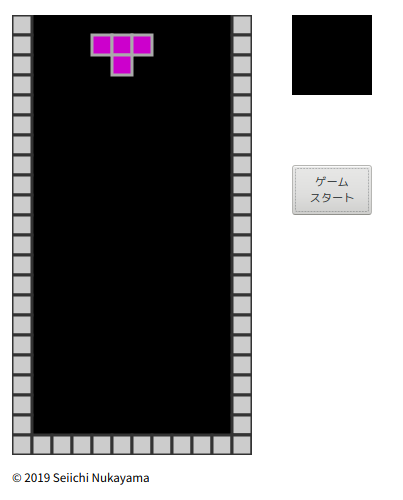
\includegraphics[width=7cm]{game4.png}

\end{document}

%% 修正時刻: Sat May  2 15:10:04 2020


%% 修正時刻: Sun Jun 21 11:53:32 2020
